\chapter{Fundamentação Teórica}
\label{chap:fund-teorica}

Neste capítulo serão apresentados as bases teóricas levantadas para este trabalho.
A disposição das seção está organizado de forma a delimitar o domínio de atuação
do trabalho, partindo da visão macro, DevOps, até a visão micro, ferramentas de
extração de configuração, que é o foco deste trabalho.

\section{DevOps}
\label{sec:devops}

O termo DevOps tem sido usado com frequência em diversas esferas do
desenvolvimento de software da atualidade, mas por ser um conceito recente
(2008), muita cunfusão ainda é gerada ao tentar definir e trabalhar com
DevOps~\cite{adambertram:2016}. ''A palavra DevOps vem de duas palavras em
inglês, \textit{development} e \textit{operations} (desenvolvimento e operações) e de maneira
geral é a cultura, movimento ou conjunto de práticas que incentiva
a comunicação, a colaboração e a integração de desenvolvedores de software
e outros profissionais de TI. Além das práticas também engloba ferramentas
e técnicas que que automatizam o processo de entrega de software e as mudanças
de infraestrutura~\cite{loukides2012devops}~\cite{erich2014mapping}.

Muitas vezes o termo é confundido com uma nova responsabilidade, ou cargo
dentro de uma empresa que desenvolve software, e por mais que seja possível
ter profissionais que tenham proficiência nas ferramentas relacionadas a
DevOps, o ideal, como dito anteriormente, é ter uma melhor comunicação,
colaboração e integração entre os times já existentes. As ferramentas
relacionadas à DevOps facilitam esses aspectos, mas o diferencial é a
mudança no processo de desenvolvimento para absorver essas melhorias
~\cite{adambertram:2016}.

A ferramenta proposta por esse Trabalho de Conclusão de Curso entra na categoria
de ferramentas DevOps que agilizam a configuração de ambientes, podendo ser ambientes
de produção ou desenvolvimento.

%TODO: parece está faltando mais alguma coisa de DevOps

\section{Metodologia Ágil}

A metodologia ágil surgiu como uma resposta às maneiras tradicionais de desenvolvimento
de software considerando uma nova abordagem com relação a práticas, organização,
documentação e foco no desenvolvimento em si.~\cite{agilemetorg:2016}

A maneira mais popular de se introduzir agilidade a um projeto é o Scrum. O Scrum
foca principalmente em retorno empírico de métricas, auto gerenciamento de
equipes e esforço para construir produtos testados de maneira 
satisfatória.~\cite{agilemetorg:2016}

\subsection{Metodologia Iterativa}

Diferentemente da metodologia de Cascata, por exemplo, o Scrum implementa uma
abordagem iterativa e incremental, podendo assim desenvolver incrementos de
maior valor pro cliente mais cedo, e assim tendo \textit{feedback} para correções
mais frequentes. A figura~\ref{fig:iterative} mostra um exemplo dessas
Iterações.~\cite{scrumreference:2016}

\begin{figure}[H]
  \centering
  \includegraphics[width=0.8\textwidth]{figuras/iterative.eps}
  \caption{Iterações do Scrum}
  \label{fig:iterative}
\end{figure}

\subsection{Papéis}

Outros tipos de metodologias ágeis possuem algumas outras características, outros
papéis, e conjuntos diferentes de práticas. O Scrum é o mais popular por sua
simplicidade~\cite{ilieva2004analyses}. Um dos pontos importantes dessa
simplicidade é a existência de somente três papéis oficiais da metodologia. O 
PO (\textit{Product Owner}, dono do produto) que é responsável por sempre dar
retorno referentes às entregas frequentes do time, pela visão do produto,
e decisões de entregas. O time de desenvolvimento Scrum, que inclui profissionais
com habilidades não tradicionais de desenvolvedores, como gerenciamento de
infraestrutura, análise de negócio ou expertize do domínio, além de
desenvolvedores clássicos. E por fim o ScrumMaster que tem responsabilidades
relacionadas à facilitar o processo do Scrum, criar um ambiente que propicie
auto organização, proteger o time de interferências que atrapalhem o seu foco e
manter as práticas ágeis e do Scrum dentro dos
padrões~\cite{scrumreference:2016}.

\subsection{Scrum Meeting}

Já que o Scrum prega a maior comunicação entre a equipe, entre si e com o cliente,
diversas reuniões são previstas na metodologia. A figura~\ref{fig:scrum_flow}
mostra o fluxo dessas reuniões.

\begin{figure}[H]
  \centering
  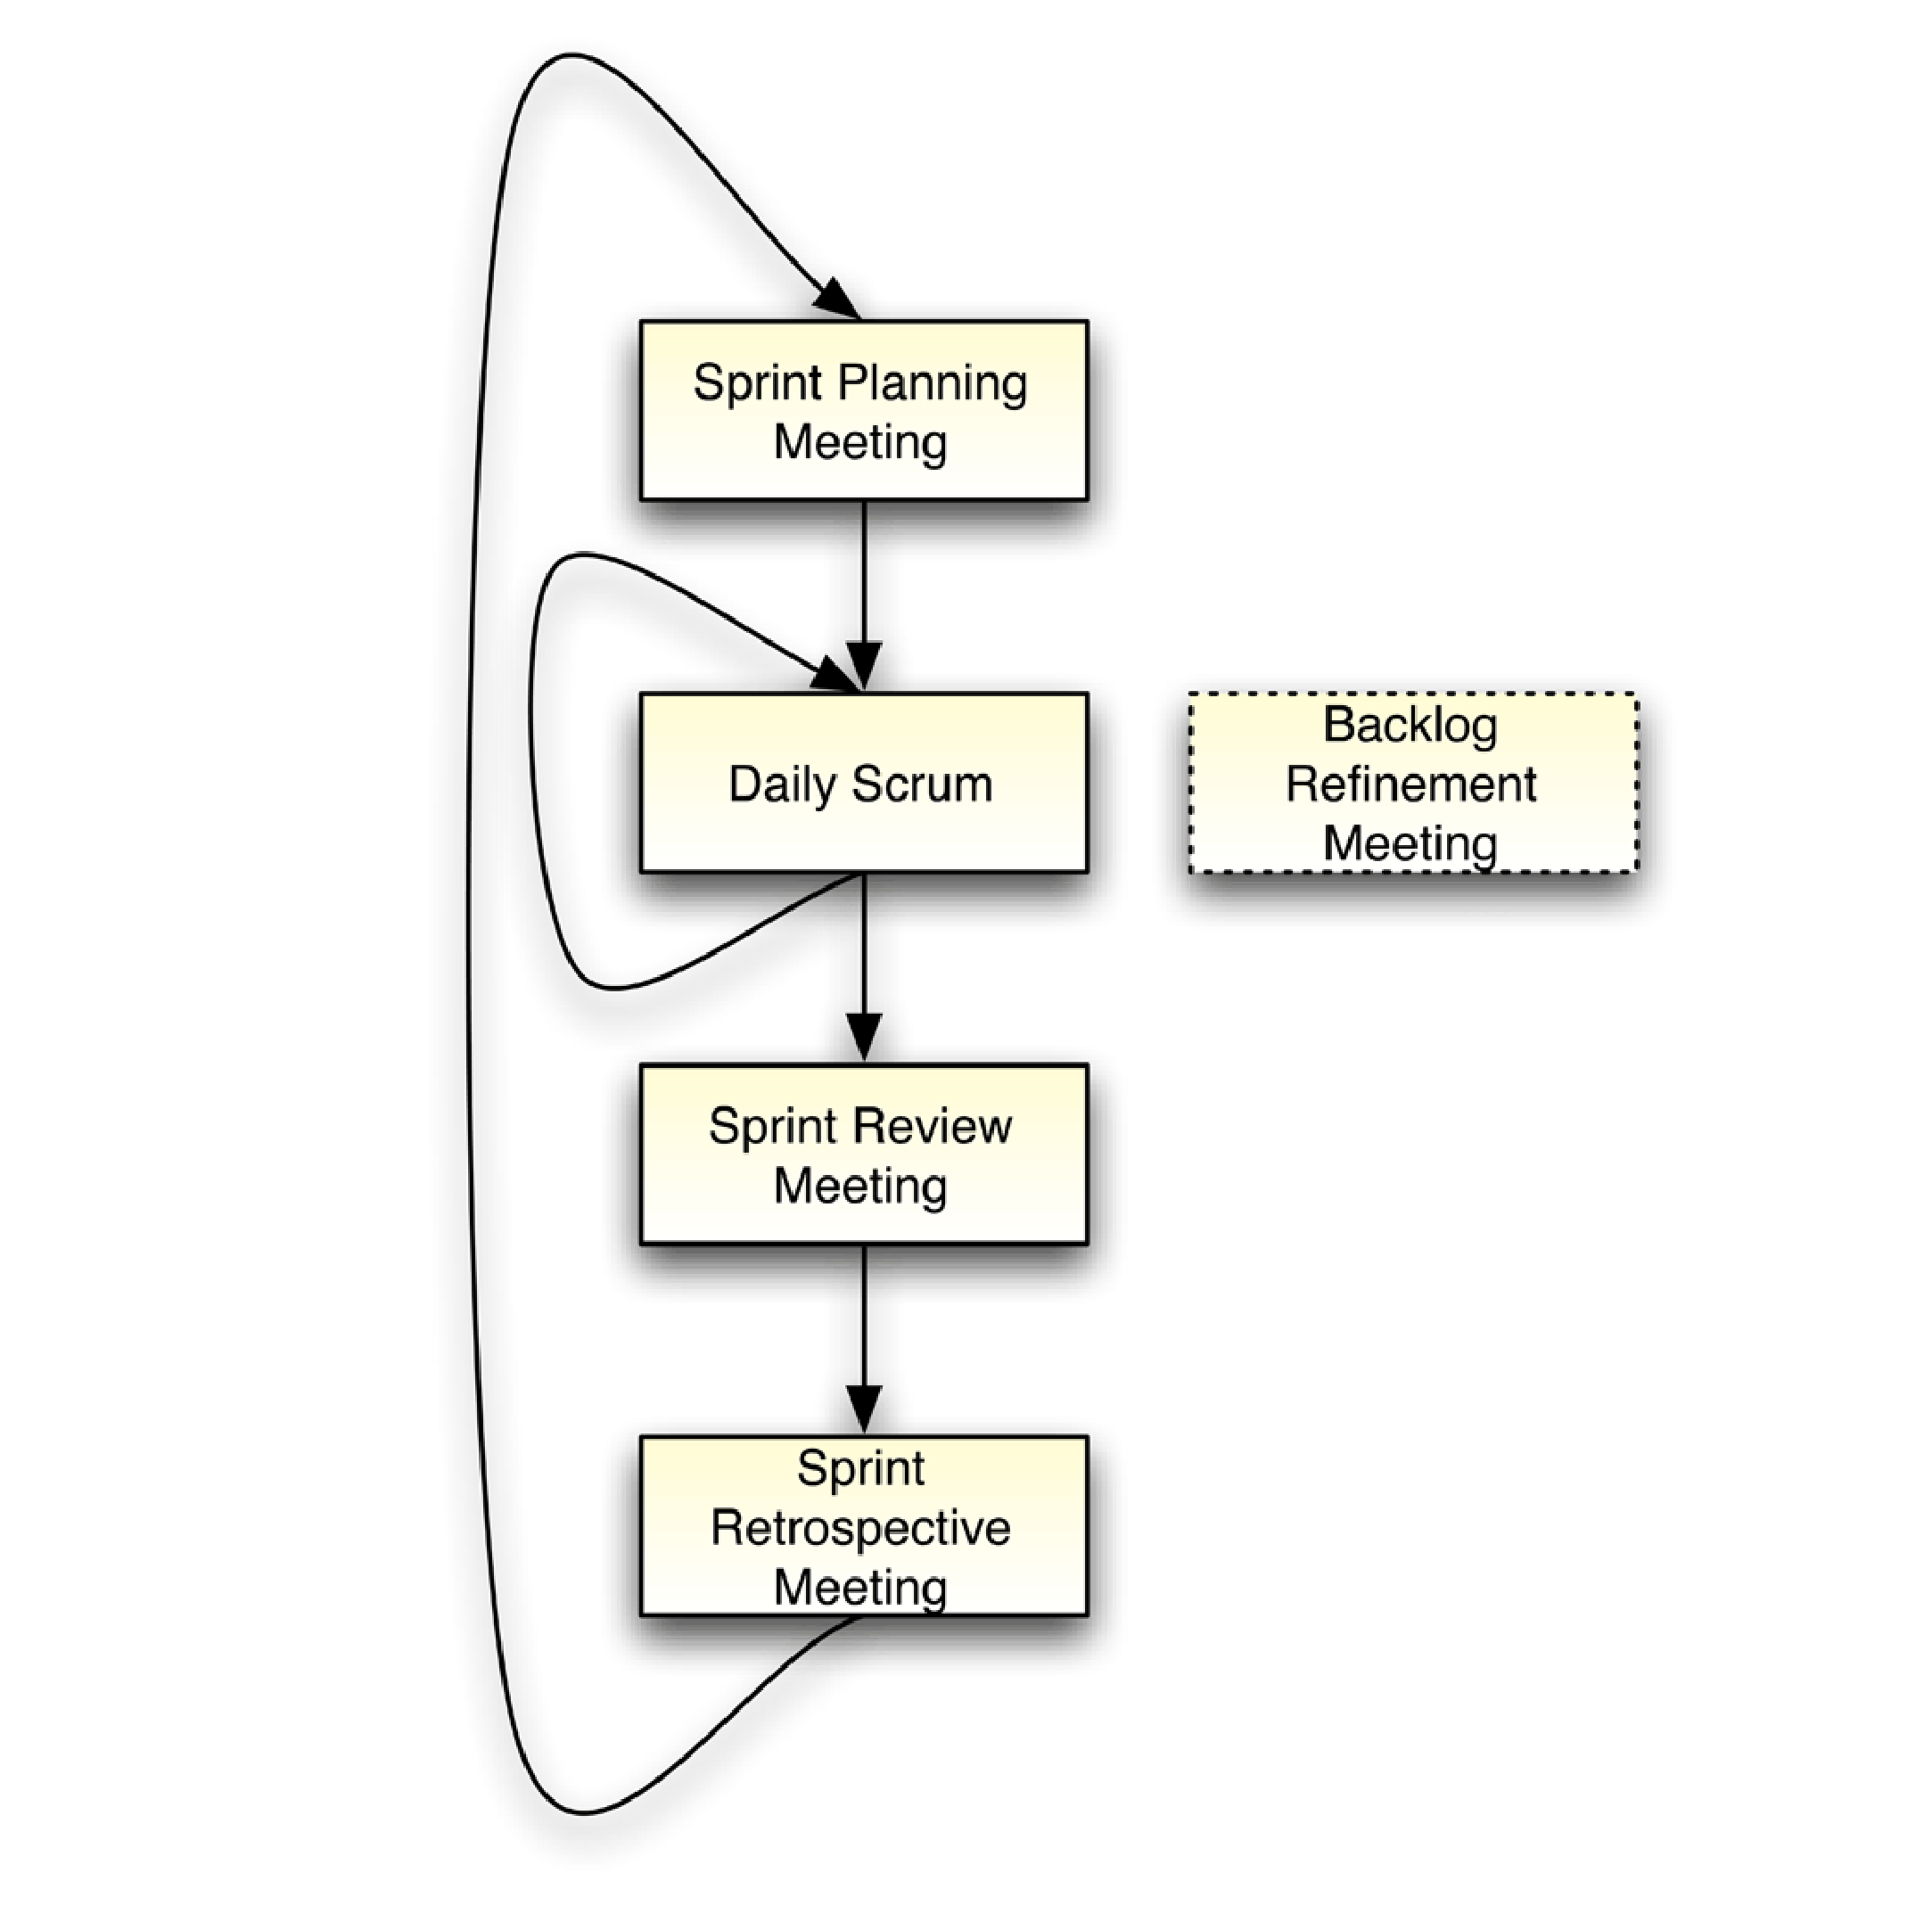
\includegraphics[width=0.8\textwidth]{figuras/scrum_flow.eps}
  \caption{Fluxo Scrum}
  \label{fig:scrum_flow}
\end{figure}

\subsection{Prática Relacionada - XP}

Um exemplo de metodologia de desenvolvimento ágil muitas vezes utilizado em
conjunto com o Scrum é a \textit{eXtreme Programming} (XP). O ScrumMaster pode
incentivar o time a utilizar práticas do XP, como integração contínua, 
desenvolvimento orientado a testes, pareamento, dentre outras.

\section{Métodos Ágeis e DevOps}

Os métodos ágeis são formas de sustentação da filosofia ágil proposta no manifesto
ágil. As duas mais populares são o \textit{Scrum} e o \textit{Extreme Programming}. Nelas
são definidas práticas que eram comumente utilizadas em outros contextos,
mas foram adaptadas para se adequarem a filosofia ágil~\cite{shore:2007}.

Com a popularização da metodologia de desenvolvimento Ágil, que tem, dentre outros
objetivos, o de entregar com maior frequência, e melhorar a comunicação entre os
times, é simples fazer a relação de DevOps com esse tipo de desenvolvimento.
DevOps nada mais é do que a implementação de conceitos e mudanças organizacionais
e culturais provenientes do pensamento Ágil \cite{scott2014}.

DevOps tenta alcançar entregas mais frequentes ao preparar um ambiente que facilite,
automatize e integre vários dos processos que antes seriam manuais, e mais
suscetíveis à falhas e atrasos, o que não é possível sem uma equipe integrada
nesse ambiente. Dessa forma, o conceito de entrega contínua e de integração
contínua estão fortemente relacionados à DevOps.~\cite{adambertram:2016}

\subsection{Integração Contínua}

Integração contínua é a prática de integrar diversas partes de um software
desenvolvido em diversas frentes, de maneira periódica, ou a cada mudança.
Foi adotado como parte da \textit{extreme programming} (XP) que sugere integrar
partes do software mais de uma vez por dia \cite{fowler2006continuous}.

Mesmo que não se adote desenvolvimento orientado a teste (TDD - test driven 
development), uma funcionalidade só está pronta se estiver com seus testes 
implementados, levando em consideração metodologias de desenvolvimento Ágil. 
E dessa forma a integração contínua pode dar retorno com relação aos resultados
desses testes a todo momento que ocorrer uma nova integração do software.

\subsection{Entrega Contínua}

A Entrega Contínua é uma prática adotada pelos métodos ágeis que tem o objetivo
de preparar um \textit{software} para que ele seja passível de ser posto em produção a
qualquer momento~\cite{olausson:2016}. 

A prática de Entrega Contínua  é frequentemente confundido com a Integração
Contínua. Existe uma relação de dependencia entre as duas práticas para
construir uma estrutura que possa sustentar a entrega contínua de um
\textit{software}.~\citeonline{olausson:2016} resume os dois em:

\begin{itemize}
  \item \textbf{Integração Contínua}: é voltada para estabelecer uma rápida
    validação da fase de desenvolvimento;
  \item \textbf{Entrega Contínua}: é voltada para estabelecer uma cultura onde
    pode-se oferecer um recurso ou \textit{feature} para o cliente a qualquer
    momento.
\end{itemize}


\section{Automação}
\label{sec:auto}

Em DevOps, a automação é um elemento essencial para se alcaçar a maturidade
de entregas e \textit{feedback} rápidos. A automação consiste na execução
automatica de um processo com o mínimo de intervensão humana. Para a área
de TI, a automação ocorre nos processos de controle e administração de
sistemas ou softwares~\cite{sharma:2015}.

Pode-se citar algumas das vantagens da automação~\cite{sharma:2015}:
\begin{itemize}
  \item Ajuda a reduzir a complexidade de um processo;
  \item Ajuda a reduzir possibilidade de erros humanos em tarefas
    repetitivas;
\end{itemize}

\citeonline{sharma:2015} aborda as necessidade de se adotar automação na área
de TI (Tecnologia da Informação) e os relaciona com conceitos métodos
ágeis, entrega contínua, computação em nuvem, etc. Além disso, são citados %TODO: falar um pouco melhor do relacionamento entre os conceitos
os benefícios da automação mapeados com as principais preocupações da industria
de TI. Algumas delas:

\begin{itemize}
  \item \textbf{Agilidade}: promove pontualidade e agilidade para a TI. Em conjunto
    com os métodos ágeis resulta em múltiplas implantações em um curto intervalo
    de tempo, além do rápido \textit{feedback};
  \item \textbf{Escalabilidade}: a automação ajuda a transformar a infraestrutura
    em códigos simples, ou seja, a construção, reconstrução e configuração é possível
    ser feita em poucos minutos. Sendo assim é possível manipular grandes quantidades
    de ambientes;
  \item \textbf{Precisão de Implantação}: com a utilização de \textit{scritps}
    é possível realizar rápidas mudanças nas configurações de um ambiente
    obtendo os resultados esperados.
\end{itemize}

A automação, em conjunto com a cultura DevOps, consegue suportar rápidas mudanças,
entrega contínua, correção de \textit{bugs}. Tudo é feito com a utilização de
código que inclui vantagens como testes, versionamento de código e
integração de aplicações~\citeonline{sharma:2015}.


\section{Infraestrutura como Código}

Segundo ~\citeonline{huttermann:2012}, em linhas gerais, o que é considerado
infraestrutura são os itens como sistema operacional, servidoes,
\textit{switches} e \textit{routers}, mas pode, também, ser a combinação
de todos os ambientes da empresa e os serviços de suporte (\textit{firewall},
sistema de monitoramento, etc).

Antes dos conceitos de DevOps e dos movimentos ágeis, as configurações de
infraestrutura eram automatizadas com \textit{scripts} que geralmente eram
difíceis de serem compreendidos por alguém que não fosse o autor~\cite{huttermann:2012}.
Recentemente, o termo Infraestrutura como Código veem se popularizando
seguindo a mesma lógica que era informalmente aplicada anteriormente, criando
\textit{scripts} de automação de configuração para a infraestrutura.

A infraestrutura como código é focada em manipular a configuração da infraestrutura
da mesma maneira que os desenvolvedores manipulam os seus códigos: escolhendo a melhor
linguagem e ferramenta para o desenvolvimentos da solução, transformando uma especificação
em algo executável que possa ser aplicada em um sistema de forma eficiente e
repetível~\cite{huttermann:2012}. \\

\noindent\begin{minipage}{.45\textwidth}
  \label{code:shell}
  \lstset{style=shell}
  \lstinputlisting[language=Bash, label=code:shell, caption="Código em Shell"]{conteudo/code/shell_example.sh}
\end{minipage}\hfill
\begin{minipage}{.45\textwidth}
  \label{code:chef}
  \lstset{style=shell}
  \lstinputlisting[language=Bash, label=code:chef, caption="Código em Chef"]{conteudo/code/chef_example.rb}
\end{minipage}


Neste trabalho será abordado a ferramenta Chef, que consiste em uma ferramenta de
automação de configuração de infraestrutura da qual utiliza o conceito de infraestrutura
como código para estabelecer os \textit{scripts} configuração. Na a representação \ref{code:shell}
\ref{code:chef} é um exemplo de um \textit{script} escrito em \textit{shell} e outro em \textit{Ruby}
interpretada pela ferramenta Chef.

\section{Ferramentas de Automação}
\label{sec:ferramenta_automacao}

%TODO: adicionar "link" entre essa seção e infraestrutura como código

\citeonline{sharma:2015} lista as ferramentas de automação que são alternativas ao
Chef. Cada qual trata a automação de uma forma diferente apresentando \textit{features} %TODO: alterar a primeira frese, pois ainda não foi descrito o Chef
específica que provê desde da automação de configuração da rede até a configuração
de ambientes. Dentre elas, destaca-se as mais populares: Chef, Puppet,
SaltStack e Ansible. A tabela~\ref{tab:chef-rival} mostra a comparação entre
as ferramentas.

\begin{table}[H]
  \centering
  \label{tab:chef-rival}
  \begin{tabular}{|l|l|l|l|l|}
    \hline
                                                                       & Chef                                                                                                                                  & Puppet                                                                                                                        & SaltStack    & Ansible                                                                                               \\ \hline
    Licença                                                            & Apache                                                                                                                                & Apache                                                                                                                        & Apache       & GPL                                                                                                   \\ \hline
  \begin{tabular}[c]{@{}l@{}}Linguagem de\\ Programação\end{tabular} & \begin{tabular}[c]{@{}l@{}}Ruby (cliente) e\\ Ruby/Erlang (servidor)\end{tabular}                                                     & Ruby                                                                                                                          & Python       & Python                                                                                                \\ \hline
    Arquitetura                                                        & Master/Agent                                                                                                                          & Master/Agent                                                                                                                  & Master/Agent & Master/Agent                                                                                          \\ \hline
  \begin{tabular}[c]{@{}l@{}}Mecanismo\\ de Push/Pull\end{tabular}   & Pull                                                                                                                                  & Pull                                                                                                                          & Push         & Push                                                                                                  \\ \hline
  Exemplo Industrial                                                 & \begin{tabular}[c]{@{}l@{}}Facebook, Linkedin, Youtube,\\ Splunk, Rackspace, GE\\ Capital, Digital Science e\\ Bloomberg\end{tabular} & \begin{tabular}[c]{@{}l@{}}Twitter, Verizon,\\ VMware, Sony, Symantec,\\ Redhat, Salesforce, Motorola\\ e Paypal\end{tabular} & Lyft         & \begin{tabular}[c]{@{}l@{}}Apple, Juniper, Grainger,\\ WeightWatchers, SaveMart\\ e NASA\end{tabular} \\ \hline
  \end{tabular}
  \caption{Comparativo das ferramentas de automação (adaptado de \citeonline{sharma:2015})}
\end{table}

%TODO: adicionar que vamos utilizar o Chef e linkar com as vantagens

As vantagens e pontos chaves que o Chef tem em relação ao seus
concorrentes~\cite{sharma:2015}:
\begin{itemize}
  \item O Chef é puramente uma \textit{Domain Specific Language (DSL)}.~\citeonline{van:2000}
    propões a definição de DSL como uma linguagem de programação executável que
    contém notações e abstrações específicas para um domínio de problemas. O Chef
    extende a sua DSL da linguagem Ruby;
  \item O Chef contém uma consistente documentação, materias de treinamento e
    atualizações constantes.
  \item O suporte da comunidade do Chef é grande e responde rapidamente a duvidas
    e problemas de instalação, configuração e utilização da ferramenta Chef.
    Além disso, constantemente publicam conferências \textit{online} e materiais multimídia
    gratuitamente.
\end{itemize}


\section{Chef}
\label{sec:chef}


\section{Ferramentas de Extração de Configuração}

\subsection{Blueprint}



